\documentclass[pdf,fyma2,final]{beamer}
\usepackage[T1]{fontenc} 
\usepackage[utf8]{inputenc}
\usepackage[czech, english]{babel}
\selectlanguage{czech}
\newcommand\tab[1][1cm]{\hspace*{#1}}
\usetheme{Warsaw}
\title{Newtonovy kroužky}
\subtitle{Semestrální projetk do předmětu FYO}
\date{\today}
\author{Patrik Chukir}
\begin{document}
	\frame{
		\maketitle
	}
	\section{Newtonovy kroužky}
	\frame{
		\frametitle{Newtonovy kroužky}
		\begin{columns}
			\begin{column}{0.5\textwidth}
				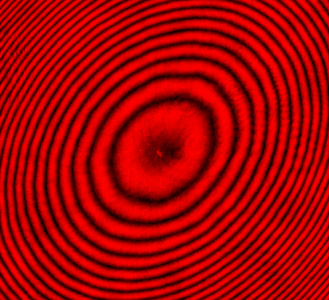
\includegraphics[width=5cm]{nr2}\\
				{\footnotesize Zdroj: Wikipedie: Newton's Rings}
			\end{column}
			\begin{column}{0.5\textwidth}  %%<--- here
				\begin{center}
					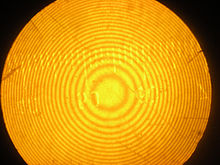
\includegraphics[width=5cm]{nr}\\
					{\footnotesize Zdroj: Wikipedie: Newton's Rings}
				\end{center}
			\end{column}
		\end{columns}
	}
	\frame{
		\frametitle{Vznik}
		%Obrázek z wiki/nebo podobnej
		%Ty dva vzorecky
				\begin{columns}
			\begin{column}{0.55\textwidth}
				\begin{itemize}
					\item Konstruktivní a destruktivní interference
					\item Vlnová délka a velikost mezery
					\item Lichý násobek poloviny $\lambda$  = Konstruktivní 
					\item Sudý násobek poloviny $\lambda$ =  Destruktivní 	
				\end{itemize}		
			\end{column}
			\begin{column}{0.5\textwidth}  %%<--- here
				\begin{center}
					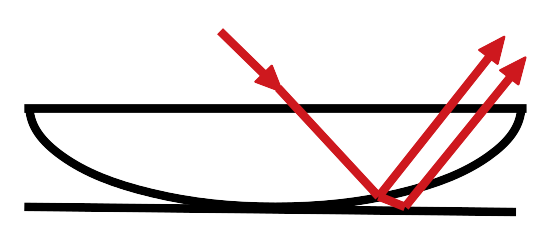
\includegraphics[width=1\textwidth]{inter}
				\end{center}
			\end{column}
		\end{columns}
	}

	\frame{
	\frametitle{Vzorec}
	\begin{itemize}
		\item Výpočet n-tého kroužku světla
		\begin{equation*}
			r_n = \sqrt{(n+\frac{1}{2}) \cdot \lambda \cdot R } 
		\end{equation*} 
		\item Výpočet n-tého neosvětleného kroužku 
		\begin{equation*}
			r_n = \sqrt{n \cdot \lambda \cdot R } 
		\end{equation*} 
		
		\item Výpočet osvětlení nad mezerou výšky g 
		\begin{equation*}
		intesity = \frac{2 \cdot g}{\lambda \cdot 0.5}
		\end{equation*} 
	\end{itemize}

	}	
	\section{Původ}
		\frame{
		\frametitle{Původ jména}
		% Issac newten a ten druhej plus rok
		\begin{columns}
			\begin{column}{0.55\textwidth}
				\begin{itemize}
					\item Poprvé popsán 1664 Robertem Hookem
					%v knize micrographia
					\item Více se jevem zabýval až Isaac Newton
					\item Jev využil pro srovnání kvality optiky teleskopu
					\item Isaac Newton jej v popsal v publikaci až 1717
				\end{itemize}		
			\end{column}
			\begin{column}{0.5\textwidth}  %%<--- here
				\begin{center}
					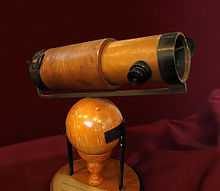
\includegraphics[width=1\textwidth]{tel}
				\end{center}
			\end{column}
		\end{columns}

		
	}
	
	\section{Využití jevu}
	\frame{
		\frametitle{Využití jevu}
						\begin{columns}
			\begin{column}{0.55\textwidth}
				\begin{itemize}
					\item Přesné měření vzdálenosti
					\item Schopnost měřit přesněji než je vlnová délka 
					\item Nutný monochromatický koheretní zdroj
				\end{itemize}		
			\end{column}
			\begin{column}{0.5\textwidth}  %%<--- here
				\begin{center}
					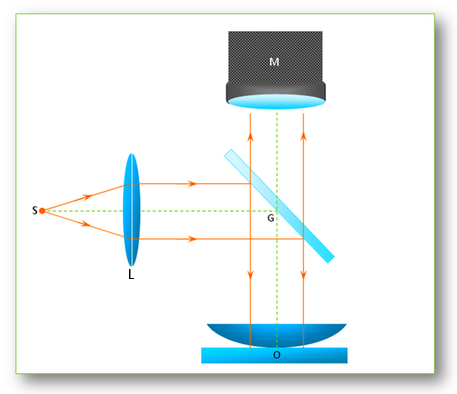
\includegraphics[width=1\textwidth]{meter}\\
					{\footnotesize Zdroj: Wikipedie: Isaac Newton}
				\end{center}
			\end{column}
		\end{columns}
	}
	\section{V přírodě}
	\frame{
	\frametitle{V přírodě}
		%bublina + olej, fotka plus mluvi o rozdílu
		\begin{columns}
			\begin{column}{0.4\textwidth}
				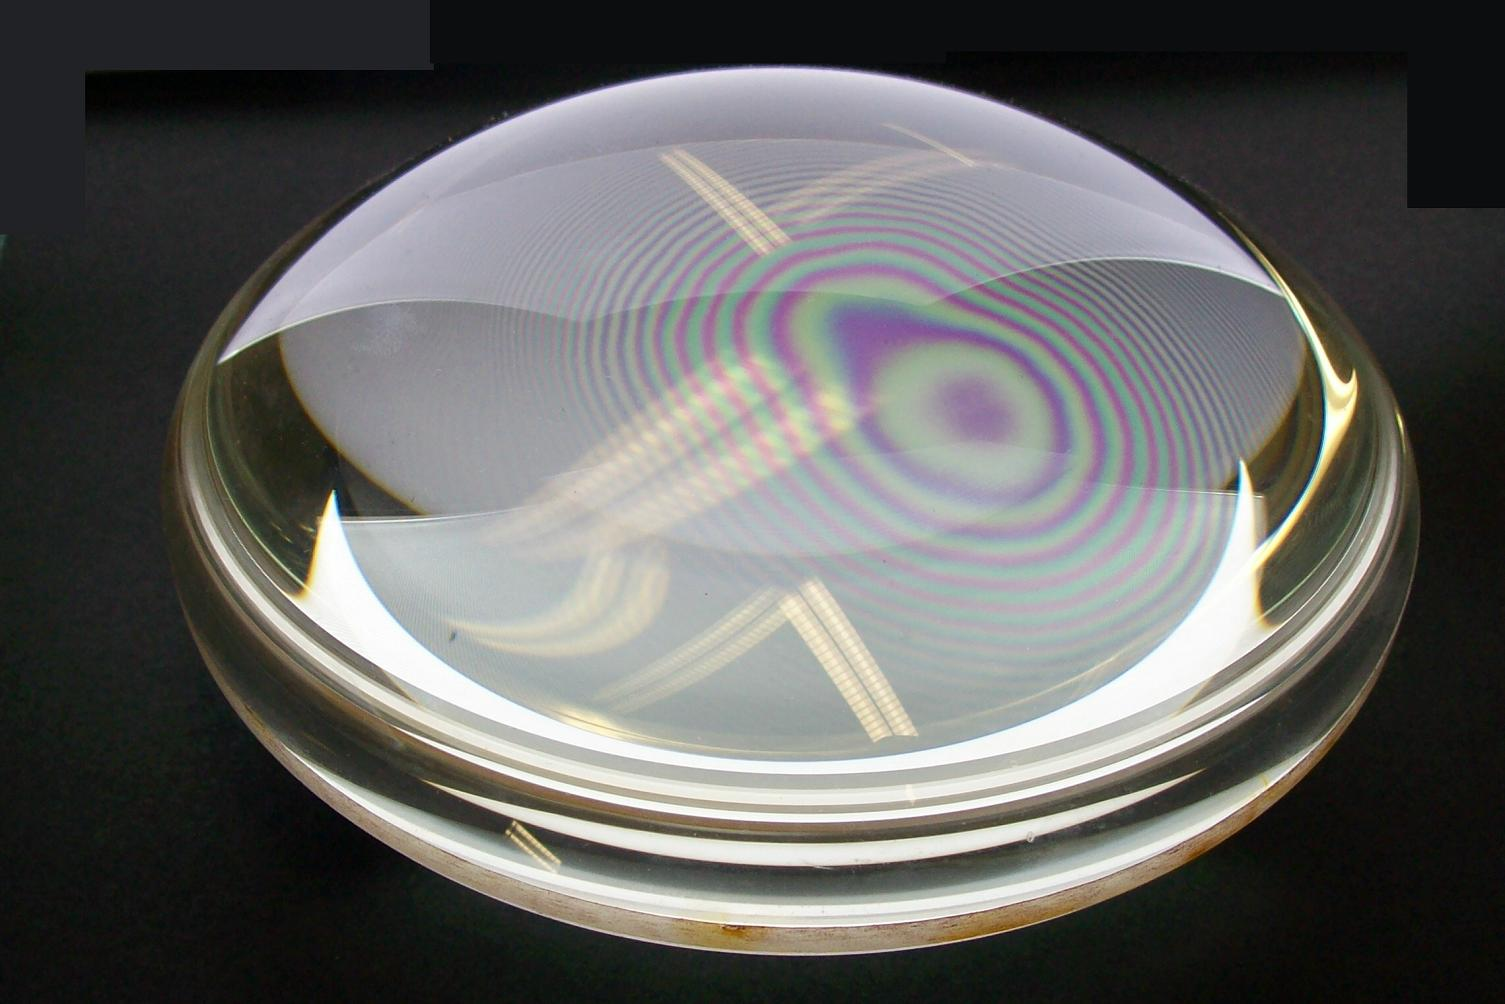
\includegraphics[width=5cm]{bub}\\
				{\footnotesize Zdroj: Wikipedie: Newton's Rings}\\
			\end{column}
			\begin{column}{0.6\textwidth}  %%<--- here
				\begin{itemize}
					\item mastnota na optické čočce
					\item Olej na hladině
					\item Duhový v důsledku bílého světla místo monochromatického
				\end{itemize}	
			\end{column}
		\end{columns}
	}
	\section{Zdroje}
\frame{
	\frametitle{Zdroje}
	\begin{enumerate}
		\small{
		\setbeamertemplate{enumerate items}[default]
	\item Wikipedie: Newton's Rings. 2018,[Online; Accesed 5-3-2018]\\
			URL: \url{https://en.wikipedia.org/wiki/Newton's_rings}
	\item Physical Optics: Newton's Rings. 2011,[Online; Accesed 5-3-2018]\\
			URL: \url{http://physical-optics.blogspot.cz/2011/06/newtons-rings.html}
	\item Hruška, P.: \textit{Fyzikální optika}. Studijní Opora,-, 2006, ISBN--
		}
	\end{enumerate}

}
\end{document}